\cmdname{EvalSimilarity} computes the similarity of two given motifs defined as a Jaccard similarity of sets of words recognized by each motif.
Optimal mutual alignment of the motifs is also estimated. Sets of recognized words are given by a PWM accompanied with threshold or a \pvalue. 

By default a set of recognized words is defined as top $0.05\%$ of words (i.e. \pvalue\ level of $0.0005$) ranked by a PWM.
It's possible to set required \pvalue\ with \cmdoption{--pvalue \requiredarg{\pvalue}} option or to specify thresholds explicitly so that word sets contain all words passing corresponding thresholds. It can be accomplished using \cmdoption{--first-threshold \requiredarg{threshold}} and \cmdoption{--second-threshold \requiredarg{threshold}}.

In order to get intuition of Jaccard similarity scale and to better catch our output format, try these examples and take a look at corresponding motif logos (see the sample data):

\exampleof{rather similar motifs \texttt{KLF4\_f2} and \texttt{SP1\_f1}, see fig.~\ref{motif-alignment-figure}}
\EvalSimilarity{motifs/KLF4\_f2.pat\\ motifs/SP1\_f1.pat}
% \outputheader
% \cmdoutputfromfile{EvalSimilarityOutput(KLF4,SP1).txt}


\begin{figure}[h]
\centering
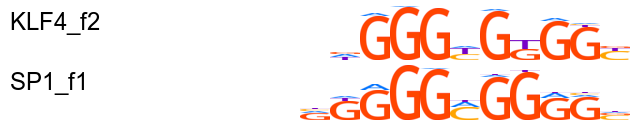
\includegraphics[width=0.9\textwidth]{./images/alignment_KLF4_SP1.png}
\caption{Sequence logo corresponding to a motif alignment.}\label{motif-alignment-figure}
\end{figure}

\exampleof{the same motif \texttt{SP1\_f1} in opposite orientations}
\EvalSimilarity{motifs/SP1\_f1\_revcomp.pat\\ motifs/SP1\_f1.pat}
% \outputheader
% \cmdoutputfromfile{EvalSimilarityOutput(SP1,revcompSP1).txt}

\exampleof{significantly different motifs \texttt{SP1\_f1} and \texttt{GABPA\_f1}}
\EvalSimilarity{motifs/SP1\_f1.pat\\ motifs/GABPA\_f1.pat}
% \outputheader
% \cmdoutputfromfile{EvalSimilarityOutput(SP1,GABPA).txt}


By default \cmdname{EvalSimilarity} tests all possible mutual motif alignments in both orientations. 
A special option \cmdoption{--position} will force evaluating similarity with the explicitly specified motif alignment:

\cmdoption{--position \requiredarg{shift},\requiredarg{direct|revcomp}}

Option parameters are comma-separated, spaces not allowed; the position is defined for the second motif relative to the first.

Try the following examples:
\exampleof{rather similar motifs \texttt{KLF4\_f2} and \texttt{SP1\_f1} at optimal alignment}
\EvalSimilarity{motifs/KLF4\_f2.pat\\ motifs/SP1\_f1.pat\\ --position -1,direct}
% \outputheader
% \cmdoutputfromfile{EvalAlignmentOutput(RightPosition).txt}

\exampleof{rather similar motifs \texttt{KLF4\_f2} and \texttt{SP1\_f1} at completely wrong alignment}
\EvalSimilarity{motifs/KLF4\_f2.pat\\ motifs/SP1\_f1.pat\\ --position 3,revcomp}
% \outputheader
% \cmdoutputfromfile{EvalAlignmentOutput(WrongPosition).txt}

{\small
\textbf{Note!} By default \cmdname{EvalSimilarity} selects the thresholds corresponding to the \pvalue\ not 
less than requested (upper boundary) possibly making compared word sets larger (not to miss words with scores too close to the threshold).
This differs from \cmdname{FindThreshold} approach which, by default, uses 
lower boundary for \pvalue thus controlling the prediction rate more strictly.

It is very important to select upper \pvalue\ boundary for short PWMs. In case of given 
low \pvalues\ they can recognize no words at all (so the Jaccard measure may have zero 
numerator and zero denominator). For reasonable threshold levels both upper and lower 
boundaries usually produce very close similarity values, see the MACRO-APE paper for details \cite{MACROAPE}.

Nevertheless, one can override this behavior with \cmdoption{‘--boundary lower’} option. In such a case if 
any of supplied PWMs recognizes no words for a selected \pvalue, then similarity can not be 
correctly determined and macroape will report the similarity value of $-1$. 
}
